\chapter{Page d'accueil}

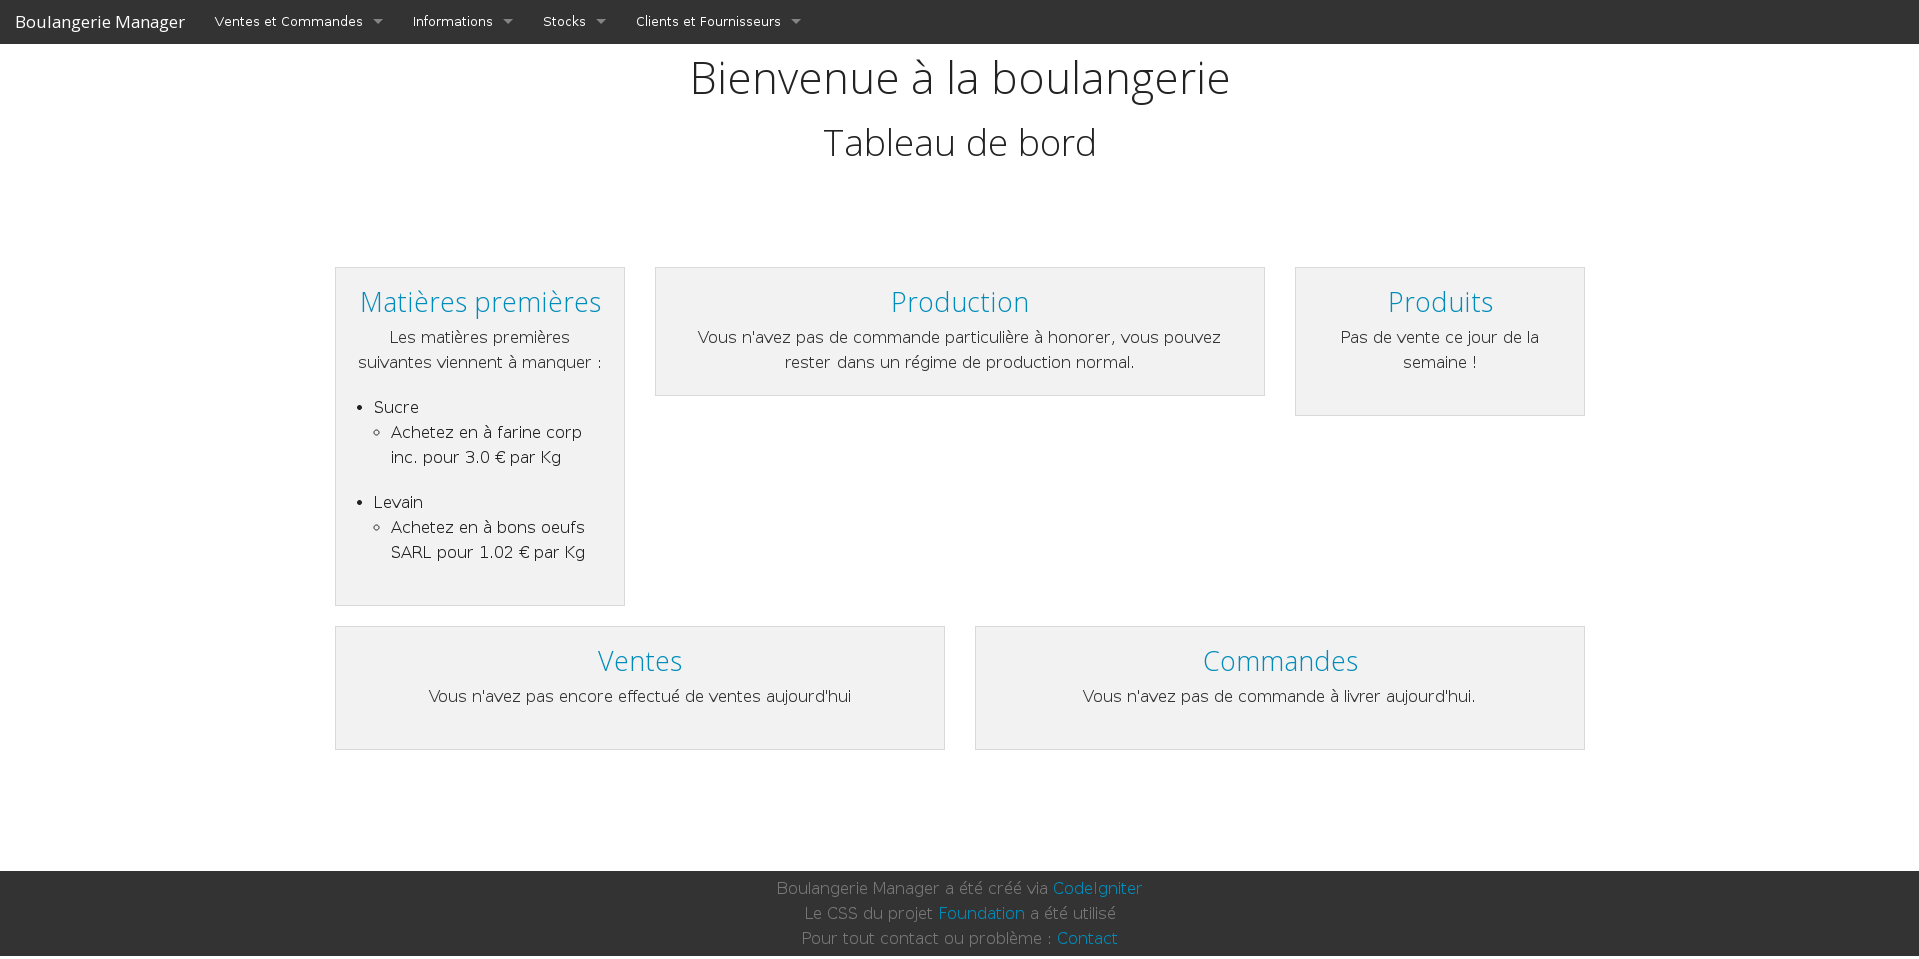
\includegraphics[scale=0.25]{homepage.png}

\paragraph{}
Voici la page d'accueil de l'application Boulangerie Manager. Elle est
présentée sous une forme de tableau de bord qui vous indique plusieurs
informations. Cette page est accessible en cliquant sur le bouton Boulangerie
Manager situé en haut à gauche de la page. Chaque rectangle concerne une
section spécifique de l'application. Voici une explication détaillée des
différentes informations que vous pourrez obtenir grâce à cette page :
\begin{enumerate}
    \item La partie Matière Première
    \begin{itemize}
        \item Cliquer sur Matière Première vous redirigera vers la partie de
            l'application consacrée aux matières premières.
        \item Les matières premières venant à manquer.
        \item Le fournisseur chez lequel vous pourrez vous procurer la matière
            première manquante au meilleur prix.
    \end{itemize}
    \item La partie Production
    \begin{itemize}
        \item Cliquer sur Production vous redirigera vers la partie de
            l'application consacrée à la production.
        \item Les informations relatives aux commandes prévues ce jour afin que
            vous puissiez gérer votre production en conséquence.
    \end{itemize}
    \item La partie Produits
    \begin{itemize}
        \item Cliquer sur Produits vous redirigera vers la partie de
            l'application consacrée aux produits.
        \item Les produits qui ont été vendus ce jour et la quantité respective
            vendue (commandes incluses).
    \end{itemize}
    \item La partie Ventes
    \begin{itemize}
        \item Cliquer sur Ventes vous redirigera vers la partie de
            l'application consacrée aux ventes.
        \item Les différents produits vendus ce jour ainsi que leur quantité
            respective.
    \end{itemize}
    \item La partie Commandes
    \begin{itemize}
        \item Cliquer sur Commandes vous redirigera vers la partie de
            l'application consacrée aux commandes.
        \item Les différentes commandes du jour.
        \item L'heure et l'adresse de livraison par commande.
    \end{itemize}
\end{enumerate}


